\documentclass{standalone}
  \usepackage{amsfonts,amsmath,amssymb}
  \usepackage[slovene]{babel}
  \usepackage[utf8]{inputenc}
  \usepackage[T1]{fontenc}
  
\usepackage{tikz, verbatim, subcaption}
\usepackage{pgfplots}
\usetikzlibrary{arrows.meta, calc, positioning, automata}

\begin{document}

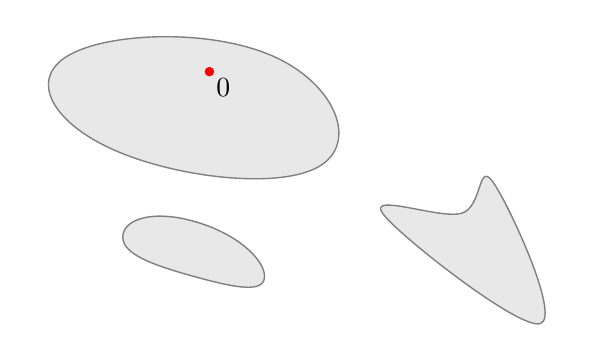
\begin{tikzpicture}
% ###############          prva slika          ###############
		\filldraw[color=gray!18] plot [smooth cycle, tension = 0.9] 
		coordinates {(-11, 6.8) (-10.4, 5.6) (-7.8, 5.4) (-8.4, 6.8)};
		\draw[gray, line width=0.5pt] plot [smooth cycle, tension = 0.9] 
		coordinates {(-11, 6.8) (-10.4, 5.6) (-7.8, 5.4) (-8.4, 6.8)};
		\filldraw[color=gray!18, line width=0.5pt] plot [smooth cycle, tension = 1.1] 
		coordinates {(-8.5, 4) (-9.4, 4.7) (-10.3, 4.5) (-9.4, 4)};
		\draw[gray, line width=0.5pt] plot [smooth cycle, tension = 1.1] 
		coordinates {(-8.5, 4) (-9.4, 4.7) (-10.3, 4.5) (-9.4, 4)};
		\filldraw[color=gray!18] plot [smooth cycle, tension = 0.7] 
		coordinates {(-6, 4.8) (-5.6, 5.2) (-5, 3.4) (-7, 4.8)};
		\draw[gray, line width=0.5pt] plot [smooth cycle, tension = 0.7] 
		coordinates {(-6, 4.8) (-5.6, 5.2) (-5, 3.4) (-7, 4.8)};
		\filldraw[red] (-9.2, 6.6) circle (1.5pt) node[black, below right=-0.5mm] {$0$};
		
\end{tikzpicture}
\end{document}